\documentclass[../main-report.tex]{subfiles}
\begin{document}
\section{Cú pháp Python cơ bản}
\subsection{Cài đặt môi trường}

Giống như các ngôn ngữ lập trình khác như Java, C++,... khi muốn chạy một
chương trình Python, trước hết cần cài đặt một môi trường có thể đọc và chạy
được Python.

Hiện phiên bản mới nhất của Python được cập nhật và dowload miễn phí trên
trang chủ python.org là Python 3.9.7.

Cùng với sự phát triển và phổ biến của Python, hiện có rất nhiều các editor có
thể được sử dụng để lập trình Python. Dựa trên kết quả đánh giá chức năng, số
lượng người dùng và phản hồi tích cực từ phía người dùng, có thể kể đến một số
phần mềm lập trình như sau:

\begin{itemize}
    \item \textbf{PyDev} - phát triển bởi Eclipse Foundation.
    \item \textbf{PyCharm} - phát triển bởi JetBrains.
    \item \textbf{Visual Studio Code} - phát triển bởi Mycrosoft.
    \item \textbf{Sublime Text} - phát triển bởi Sublime HQ.
    \item \textbf{Spyder} - phát triển bởi Pierre Raybaut, chuyên dùng để lập trình khoa học.
\end{itemize}

\subsection{Biến}
Biến chính xác như tên gọi của nó, tức là giá trị của nó có thể thay đổi. Các 
biến có thể giúp lưu trữ bất cứ cái gì nếu có thể định nghĩa được nó. Các biến chỉ là 
một phần của bộ nhớ máy tính nơi lưu trữ một số thông tin. 

Xác định kiểu dữ liệu của biến bằng lệnh type(biến).

Có kiểu biến toàn cục và biến địa phương, biến được khai báo ngoài hàm là biến
toàn cục còn biến được khai báo trong hàm là biến địa phương.

\begin{example}
Ví dụ về khai báo biến:

\begin{lstlisting}[language=Python]
    # Biến toàn cục
    x = 5
    def function():
        # biến cục bộ
        x = 10.5
        print(x)
\end{lstlisting}
\end{example}

\subsection{Toán tử}
Về cơ bản trong Python cũng có các toán tử số học, quan hệ, logic...tương tự như các ngôn ngữ
khác.

\begin{itemize}
\item \textbf{Toán tử số học}
\begin{table}[ht!]
\centering
\begin{tabular}{|>{\centering\arraybackslash}p{2cm}|>{\centering\arraybackslash}p{5cm}|>{\centering\arraybackslash}p{5cm}|}
\hline
\textbf{Toán tử} & \textbf{Mô tả}             & \textbf{Ví dụ: a=20, b=10} \\ \hline
+                & Phép cộng                  & $a+b=30$                   \\ \hline
\-               & Phép trừ                   & $a-b=10$                   \\ \hline
*                & Phép nhân                  & $a*b=200$                  \\ \hline
/                & Phép chia lấy phần nguyên. & $a/b=2$                    \\ \hline
\%               & Phép chia lấy phần dư.     & $a\:\%\:b=0$                   \\ \hline
**               & Phép lấy số mũ             & $a\:**\:b=10^{20}$            \\ \hline
//               & Floor Division             & $9//2=4$                   \\ \hline
\end{tabular}
\caption{Toán tử số học}
\label{tab:toán tử số học}
\end{table}

\item \textbf{Toán tử quan hệ}
\begin{table}[ht!]
\centering
\begin{tabular}{|>{\centering\arraybackslash}p{2cm}|>{\centering\arraybackslash}p{5cm}|>{\centering\arraybackslash}p{5cm}|}
\hline
\textbf{Toán tử} & \textbf{Mô tả}             & \textbf{Ví dụ: a=20, b=10} \\ \hline
$==$             & So sánh bằng               & $(a==b)$ cho kết quả False \\ \hline
$!=$             & So sánh không bằng.        & $(a!=b)$ cho kết quả True.  \\ \hline
$<>$             & Không bằng                 & $(a<>b)$ cho kết quả True.   \\ \hline
$>$              & Lớn hơn.                   & $(a>b)$ cho kết quả True.    \\ \hline
$<$              & Nhỏ hơn.                   & $(a<b)$ cho kết quả False   \\ \hline
$>=$             & Lớn hơn hoặc bằng.         & $(a>=b)$ cho kết quả True   \\ \hline
$<=$             & Nhỏ hơn hoặc bằng.         & $(a<=b)$ cho kết quả False    \\ \hline
\end{tabular}
\caption{Toán tử quan hệ}
\label{tab:toán tử quan hệ}
\end{table}

\item \textbf{Toán tử logic}
\begin{table}[ht!]
\centering
\begin{tabular}{|>{\centering\arraybackslash}p{2cm}|>{\centering\arraybackslash}p{5cm}|>{\centering\arraybackslash}p{5cm}|}
\hline
\textbf{Toán tử} & \textbf{Mô tả}             & \textbf{Ví dụ: a=10, b=20} \\ \hline
and             & Nếu cả 2 biểu thưc là True thì cho kết quả True.               & $(a>9\:and\:b>19) => True$  \\ \hline
or             & Nếu 1 trong 2 là True thì cho kết quả True.        & $(a>9\:or\:b>100) => True$  \\ \hline
not             & Được sử dụng phủ định logic của biểu thức.                 & $not\: (a>9) => False$ cho kết quả True.   \\ \hline
\end{tabular}
\caption{Toán tử logic}
\label{tab:toán tử logic}
\end{table}

\item \textbf{Toán tử gán}
\begin{table}[ht!]
\centering
\begin{tabular}{|>{\centering\arraybackslash}p{2cm}|>{\centering\arraybackslash}p{5cm}|>{\centering\arraybackslash}p{5cm}|}
\hline
\textbf{Toán tử} & \textbf{Mô tả}             & \textbf{Ví dụ} \\ \hline
$=$             & Phép gán bằng.             & $c = a + b$ gán $a+b$ cho c \\ \hline
$+=$             & Phép gán cộng.             & $c += a <=> c=c+a$  \\ \hline
$-=$             & Phép gán trừ.               & $c\:-=a <=> c=c-a$  \\ \hline
$*=$              & Phép gán nhân.                  & $c\:*=a <=> c=c*a$    \\ \hline
$/=$              & Phép gán chia lấy phần nguyên.   & $c\:/=a <=> c=c/a$   \\ \hline
$\%=$             & Phép gán chia lấy phần dư.         & $c\:\%=a <=> c=c\%a$  \\ \hline
$**=$             & Phép gán lũy thừa.         & $c\:**=a <=> c=c**a$   \\ \hline
$//=$             & Phép gán chia floor.       & $c\://=a <=> c=c//a$   \\ \hline
\end{tabular}
\caption{Toán tử gán}
\label{tab:Toán tử gán}
\end{table}

\item \textbf{Toán tử khai thác}
\begin{table}[ht!]
\centering
\begin{tabular}{|>{\centering\arraybackslash}p{2cm}|>{\centering\arraybackslash}p{6cm}|}
\hline
\textbf{Toán tử} & \textbf{Mô tả}             \\ \hline
in             & Trả về true nếu tìm thấy biến a trong tập các giá trị sau in, ngược lại trả về false.                 \\ \hline
not in             & Trả về false nếu tìm thấy biến a trong tập các giá trị sau in, ngược lại trả về false.          \\ \hline
\end{tabular}
\caption{Toán tử khai thác}
\label{tab:toán tử khai thác}
\end{table}

\item \textbf{Toán tử nhận dạng} : is và not is
\begin{table}[ht!]
\centering
\begin{tabular}{|>{\centering\arraybackslash}p{2cm}|>{\centering\arraybackslash}p{6cm}|}
\hline
\textbf{Toán tử} & \textbf{Mô tả}             \\ \hline
is             & Kiểm tra xem hai giá trị có bằng nhau hay không. Toán tử này sẽ trả về True nếu a == b và ngược lại                 \\ \hline
not is            & Ngược lại của is.          \\ \hline
\end{tabular}
\caption{Toán tử nhận dạng}
\label{tab:toán tử nhận dạng}
\end{table}

\item \textbf{Toán tử thao tác bit}
\begin{table}[ht!]
\centering
\begin{tabular}{|>{\centering\arraybackslash}p{2cm}|>{\centering\arraybackslash}p{5cm}|}
\hline
\textbf{Toán tử} & \textbf{Mô tả}        \\ \hline
$\&$             & AND                  \\ \hline
$|$             & OR                      \\ \hline
\textasciicircum          & XOR                    \\ \hline
\textasciitilde             & NOT                    \\ \hline
$<<$              & Dịch trái nhị phân   \\ \hline
$>>$             & Dịch phải nhị phân       \\ \hline
\end{tabular}
\caption{Toán tử thao tác bit}
\label{tab:Toán tử thao tác bit}
\end{table}
\end{itemize} 

\textbf{Thứ tự ưu tiên của các toán tử}: Việc áp dụng nhiều toán tử trong một câu lệnh cần được chú ý đến thứ tự ưu tiên
của các toán tử đó. Theo thứ tự ưu tiên giảm dần như sau: toán tử số học, toán tử
thao tác bit, toán tử quan hệ, toán tử gán, toán tử identify, toán tử membership,
toán tử logic.

\subsection{Các kiểu dữ liệu}
Python cũng hỗ trợ các kiểu dữ liệu căn bản như:char, string, int, float, double... Ngoài ra Python cung cấp
một loạt các dữ liệu phức hợp, thường được gọi là các chuỗi (sequence), sử dụng để nhóm các
giá trị khác nhau như list, set , tuple và dictionary. Áp dụng hợp lý các kiểu dữ liệu này có thể
khiến việc lập trình nhanh hơn rất nhiều.

\begin{itemize}
\item \textbf{List}: Đây là kiểu dữ liệu được đánh giá là đa năng nhất. List được biểu diễn bằng dãy các giá trị, được phân tách nhau bằng dấu phẩy, nằm trong dấu []. List không giới hạn số lượng mục, có thể có nhiều kiểu dữ liệu khác nhau trong cùng một list, như chuỗi, số nguyên, số thập phân,...

Các giá trị trong list có chỉ số, có thứ tự, có thể thay đổi và cho phép lặp lại.
    \begin{example}
    Khai báo và sử dụng kiểu dữ liệu danh sách:
    \begin{lstlisting}[language=Python]
    list1 = [1, 2, 3.5, 10]
    list2 = [1, 1, 'hello', 'my list', 10.1, True]
    \end{lstlisting}
    \end{example}

\item \textbf{Tuple}: Tuple trong Python là một chuỗi các phần tử có thứ tự giống như list. Sự khác
biệt giữa list và tuple là không thể thay đổi các phần tử trong tuple khi đã gán,
nhưng trong list có thể thay đổi.

Tuple thường được sử dụng cho các dữ liệu không cho phép sửa đổi và
nhanh hơn list vì nó không thể thay đổi tự động.

    \begin{example}
    Ví dụ về kiểu dữ liệu tuple:
    \begin{lstlisting}[language=Python]
    mytuple = ("apple", "banana", "cherry")
    mytuple = (1, 1, 2, 3.5, 5, "hello")
    \end{lstlisting}
    \end{example}

\item \textbf{Set} : Set trong Python là tập hợp các phần tử duy nhất, không có thứ tự. Các phần tử
trong set phân cách nhau bằng dấu phẩy và nằm trong dấu ngoặc nhọn {}. Các
phần tử trong set có thể thay đổi.

    \begin{example}
    Ví dụ về kiểu dữ liệu set:
    \begin{lstlisting}[language=Python]
        set1 = {"apple", "banana", "cherry"}
        set2 = {1, 5, 7, 9, 3}
        set3 = {True, False, False}
    \end{lstlisting}
    \end{example}

\item \textbf{Dictionary}: Dictionary là tập hợp các cặp khóa giá trị không có thứ tự. Các dictionary được
tối ưu hóa để trích xuất dữ liệu với điều kiện phải biết được khóa để lấy giá trị.
Trong Python, dictionary được định nghĩa trong dấu ngoặc nhọn {} với mỗi
phần tử là một cặp theo dạng key:value. Key và value này có thể là bất kỳ kiểu
dữ liệu nào.

    \begin{example}
    Ví dụ về kiểu dữ liệu dictionary:
    \begin{lstlisting}[language=Python]
        thisdict = {
            "brand": "Ford",
            "model": "Mustang",
            "year": 1964
          }
    \end{lstlisting}
    \end{example}

\end{itemize}

\subsection{Hàm}
Trong Python, hàm là một nhóm các lệnh có liên quan đến nhau được dùng để
thực hiện một tác vụ, nhiệm vụ cụ thể nào đó. Hàm giúp chia chương trình thành
những khối/phần/module nhỏ hơn.

\begin{itemize}
\item Khi khởi tạo hàm không có kiểu dữ liệu trả về tuy nhiên ta vẫn có thể dùng lệnh return để
trả về giá trị xác định.

\item Các tham số mặc định của hàm là các tham số không bắt buộc phải cung cấp khi gọi hàm
và khi đó giá trị của nó là giá trị mặc định. Sử dụng tham số mặc định bằng cách dùng
toán tử =.

\item Tham số tùy biến sử dụng khi ta không biết trước số lượng tham số sẽ truyền vào hàm.
Khi đó biến có thể coi như một mảng các giá trị. Sử dụng tham số tùy biến bằng cách đặt
dấu * trước tên tham số.
\end{itemize}

\begin{example}
Ví dụ về khai báo và định nghĩa hàm:
\begin{lstlisting}[language=Python]
a = "Hello"

def Hello(a):
    print(a + "World")    # Hello World
\end{lstlisting}
\end{example}

\subsection{Lập trình hướng đối tượng (OOP): Class}
Python là một ngôn ngữ lập trình hỗ trợ hướng đối tượng tương tự như Java, C++, PHP... Nó
cũng có các nguyên lý cơ bản của một ngôn ngữ hướng đối tượng đó là tính đóng gói, tính kế
thừa, tính đa hình.

Hầu hết mọi thứ trong Python đều là một object, với tính chất và phương thức của riêng nó.

Class chính là một kiểu dữ liệu đặc biệt, dùng để tạo nên một đối tượng.
\begin{example}
Ví dụ về khai báo một class:
\begin{lstlisting}[language=Python]
class MyClass:
    x = 5
\end{lstlisting}
\end{example}

Chúng ta có thể tạo một đối tượng từ class đã tạo:
\begin{example}
Tạo một đối tượng p1, và in ra giá trị của x:
\begin{lstlisting}[language=Python]
p1 = MyClass()
print(p1.x)
\end{lstlisting}
\end{example}

\section*{Hàm \_\_init\_\_()}
Để hiểu rõ hơn ý nghĩa của class ta cần hiểu về hàm \_\_init\_\_(). Mỗi classes đều có một hàm \_\_init\_\_(), hàm này sẽ được thực thi ngay khi class được bắt đầu.

Ta sử dụng hàm \_\_init\_\_() để gán gía trị, thuộc tính và các thao tác cần thiết khi đối tượng được tạo.
\begin{example}
Tạo một class Person, sử dụng hàm \_\_inti\_\_() để gán tên và tuổi:
\begin{lstlisting}[language=Python]
class Person:
    def __init__(self, name, age):
        self.name = name
        self.age = age

p1 = Person("John", 36)

print(p1.name)  # John
print(p1.age)   # 36
  
\end{lstlisting}
\end{example}

\section*{Phương thức của đối tượng}
Mỗi đối tượng có thể có các phương thức. Phương thức là những hàm thuộc về đối tượng ấy.

\begin{example}
Tạo phương thức in ra lời chào, và sử dụng nó trên đối tượng p1:
\begin{lstlisting}[language=Python]
class Person:
    def __init__(self, name, age):
        self.name = name
        self.age = age

    def myfunc(self):
        print("Hello my name is " + self.name)

p1 = Person("John", 36)
p1.myfunc()
\end{lstlisting}
\end{example}

\section{Một số thư viện của Python}
Do hạn chế trong việc trình bày báo cáo nên em chỉ nêu một số ý chính của các thư viện và một số ví dụ. Các thao tác với thư viện đầy đủ hơn em đặt ở trong các file jupyter notebook của riêng từng thư viện.
\subsection{Numpy}
Numpy (viết tắt của “Numeric Python” hoặc “Numerical Python”) là một thư
viện lõi phục vụ cho khoa học máy tính của Python, hỗ trợ cho việc tính toán các mảng
nhiều chiều, có kích thước lớn với các hàm đã được tối ưu áp dụng lên các mảng nhiều
chiều đó. Numpy đặc biệt hữu ích khi thực hiện các hàm liên quan tới Đại Số Tuyến Tính.

Để cài đặt numpy, ta có 2 cách:
\begin{itemize}
    \item Sử dụng Command Prompt: 
    \begin{lstlisting}
        pip install numpy
    \end{lstlisting}
    \item Hoặc sử dụng Anaconda Prompt:
    \begin{lstlisting}
        conda install numpy
    \end{lstlisting}
\end{itemize}

\begin{itemize}
\item \textbf{Khai báo thư viện}: 
\begin{lstlisting}[language=Python] 
import numpy as np
\end{lstlisting}
\item \textbf{Khởi tạo mảng} : Numpy cho phép ta tạo các mảng 1 chiều hay nhiều chiều với nhiều cách thức khác nhau.

\begin{example}
    Một số cách tạo mảng:
\begin{lstlisting}[language=Python] 
    # Tạo mảng 1 chiều
    a = np.array([1, 2, 3, 4])   # a =  [1 2 3 4]

    # Mảng 2 chiều(nhiều chiều)
    b = np.array([[1, 2, 3, 4], [5, 6, 7, 8]])   # b =  [[1 2 3 4]
                                                 #       [5 6 7 8]]

    # Tạo mảng với các giá trị chưa biết nhưng đã biết kích thước
    d = np.zeros((3, 4))

\end{lstlisting}
\end{example}
\item \textbf{Các thao tác với mảng} : Numpy cho phép ta thực hiện các thao tác với mảng như: thực hiện các phép toán giữa các mảng, giữa các giá trị trên mảng, index, slicing, điều khiển kích thước của mảng, ...
\begin{example}
Một vài ví dụ:
\begin{lstlisting}[language=Python]
A = np.array([[1, 1], 
              [0, 1]])

B = np.array([[2, 0],
              [3, 4]])

arr1 = A * B          # Phép nhân theo từng phần tử
arr2 = A @ B          # Phép nhân ma trận. Cách khác: A.dot(B)
A *= 3                # Nhân mỗi phần tử của A với 3
A.sum(axis=1)         # Tổng các phần tử của A theo hàng

\end{lstlisting}
\end{example}
\end{itemize}

\subsection{Pandas}
Thư viện pandas trong python là một thư viện mã nguồn mở, hỗ trợ đắc lực trong
thao tác dữ liệu. Đây cũng là bộ công cụ phân tích và xử lý dữ liệu mạnh mẽ của ngôn
ngữ lập trình python. Thư viện này được sử dụng rộng rãi trong cả nghiên cứu lẫn phát
triển các ứng dụng về khoa học dữ liệu. Thư viện này sử dụng một cấu trúc dữ liệu riêng
là Dataframe. Pandas cung cấp rất nhiều chức năng xử lý và làm việc trên cấu trúc dữ liệu
này.

Để cài đặt pandas, ta có 2 cách:
\begin{itemize}
    \item Sử dụng Command Prompt: 
    \begin{lstlisting}
        pip install pandas
    \end{lstlisting}
    \item Hoặc sử dụng Anaconda Prompt:
    \begin{lstlisting}
        conda install pandas
    \end{lstlisting}
\end{itemize}

\begin{itemize}
\item \textbf{Khai báo thư viện}: 
\begin{lstlisting}[language=Python] 
import pandas as pd
\end{lstlisting}

\item \textbf{Khởi tạo}
Pandas có 2 cấu trúc dữ liệu cơ bản là: Series (1 chiều) và DataFrame (2
chiều)

Có nhiều cách để tạo một cấu trúc dữ liệu trên pandas như: truyền trực tiếp giá trị, lấy từ mảng trên Numpy, từ file, ...

\begin{example}
Một số cách tạo một cấu trúc dữ liệu trên pandas:
\begin{lstlisting}[language=Python]
# Tạo một series
series = pd.Series([1, 2, 4, 5, 7, 9, np.nan])

# Tạo DataFrame bằng cách truyền giá trị từ cấu trúc dữ liệu dictionary trong python
df2 = pd.DataFrame({
    "A" : [1, 2, 1, 2],
    "B" : pd.Timestamp("20130102"),
    "C" : pd.Series(1, index=list(range(4)), dtype="float32"),
    "D" : np.array([3]*4, dtype='int32'),
    "E" : pd.Categorical(["test", "train", "validation", "test"]),
    "F" : "Foo"
})
\end{lstlisting}
\end{example}

\item \textbf{Xem xét, lấy dữ liệu từ cấu trúc dữ liệu}
Pandas cho phép ta thao tác một cách trực quan, đơn giản với các cấu trúc dữ liệu. Ta có in ra dữ liệu, thêm, xóa, thay đổi, thống kê, chọn từng phần dữ liệu,... Ta cũng có thể lưu các dạng cấu trúc dữ liệu trên \
pandas thành các định dạng file khác nhau như csv, hdf5, ...

\begin{example}
Một số thao tác với dữ liệu:
\begin{lstlisting}[language=Python]
df.head()              # Xem 10 hàng đầu tiên của dữ liệu
df.index               # Xem các tên chỉ số 
df.columns             # Xem các cột
df.to_numpy()          # chuyển từ DataFrame sang mảng trong Numpy
df.describe()          # Hiển thị thống kê của dữ liệu
\end{lstlisting}
\end{example}
\end{itemize}

\subsection{Matplotlib}
Matplotlib là một thư viện của Python được sử dụng để vẽ đồ thị với sự trợ giúp của các thư viện khác như Numpy và Pandas.
Nó được sử dụng để tạo ra các nhiễu thống kê(statistical interferences, xuất hiện khi hai phân phối xác xuất trùng lặp lên nhau) và vẽ đồ thị
2D của các mảng. Matplotlib sử dụng pyplot để cung cấp giao diện tương tự như MATLAB và là một mã nguồn mở.
Để cài đặt matplotlib, ta có 2 cách:
\begin{itemize}
    \item Sử dụng Command Prompt: 
    \begin{lstlisting}
        pip install matplotlib
    \end{lstlisting}
    \item Hoặc sử dụng Anaconda Prompt:
    \begin{lstlisting}
        conda install matplotlib
    \end{lstlisting}
\end{itemize}

Các thành phần trong đồ thị của Matplotlib:
\begin{figure}[ht!]
\centering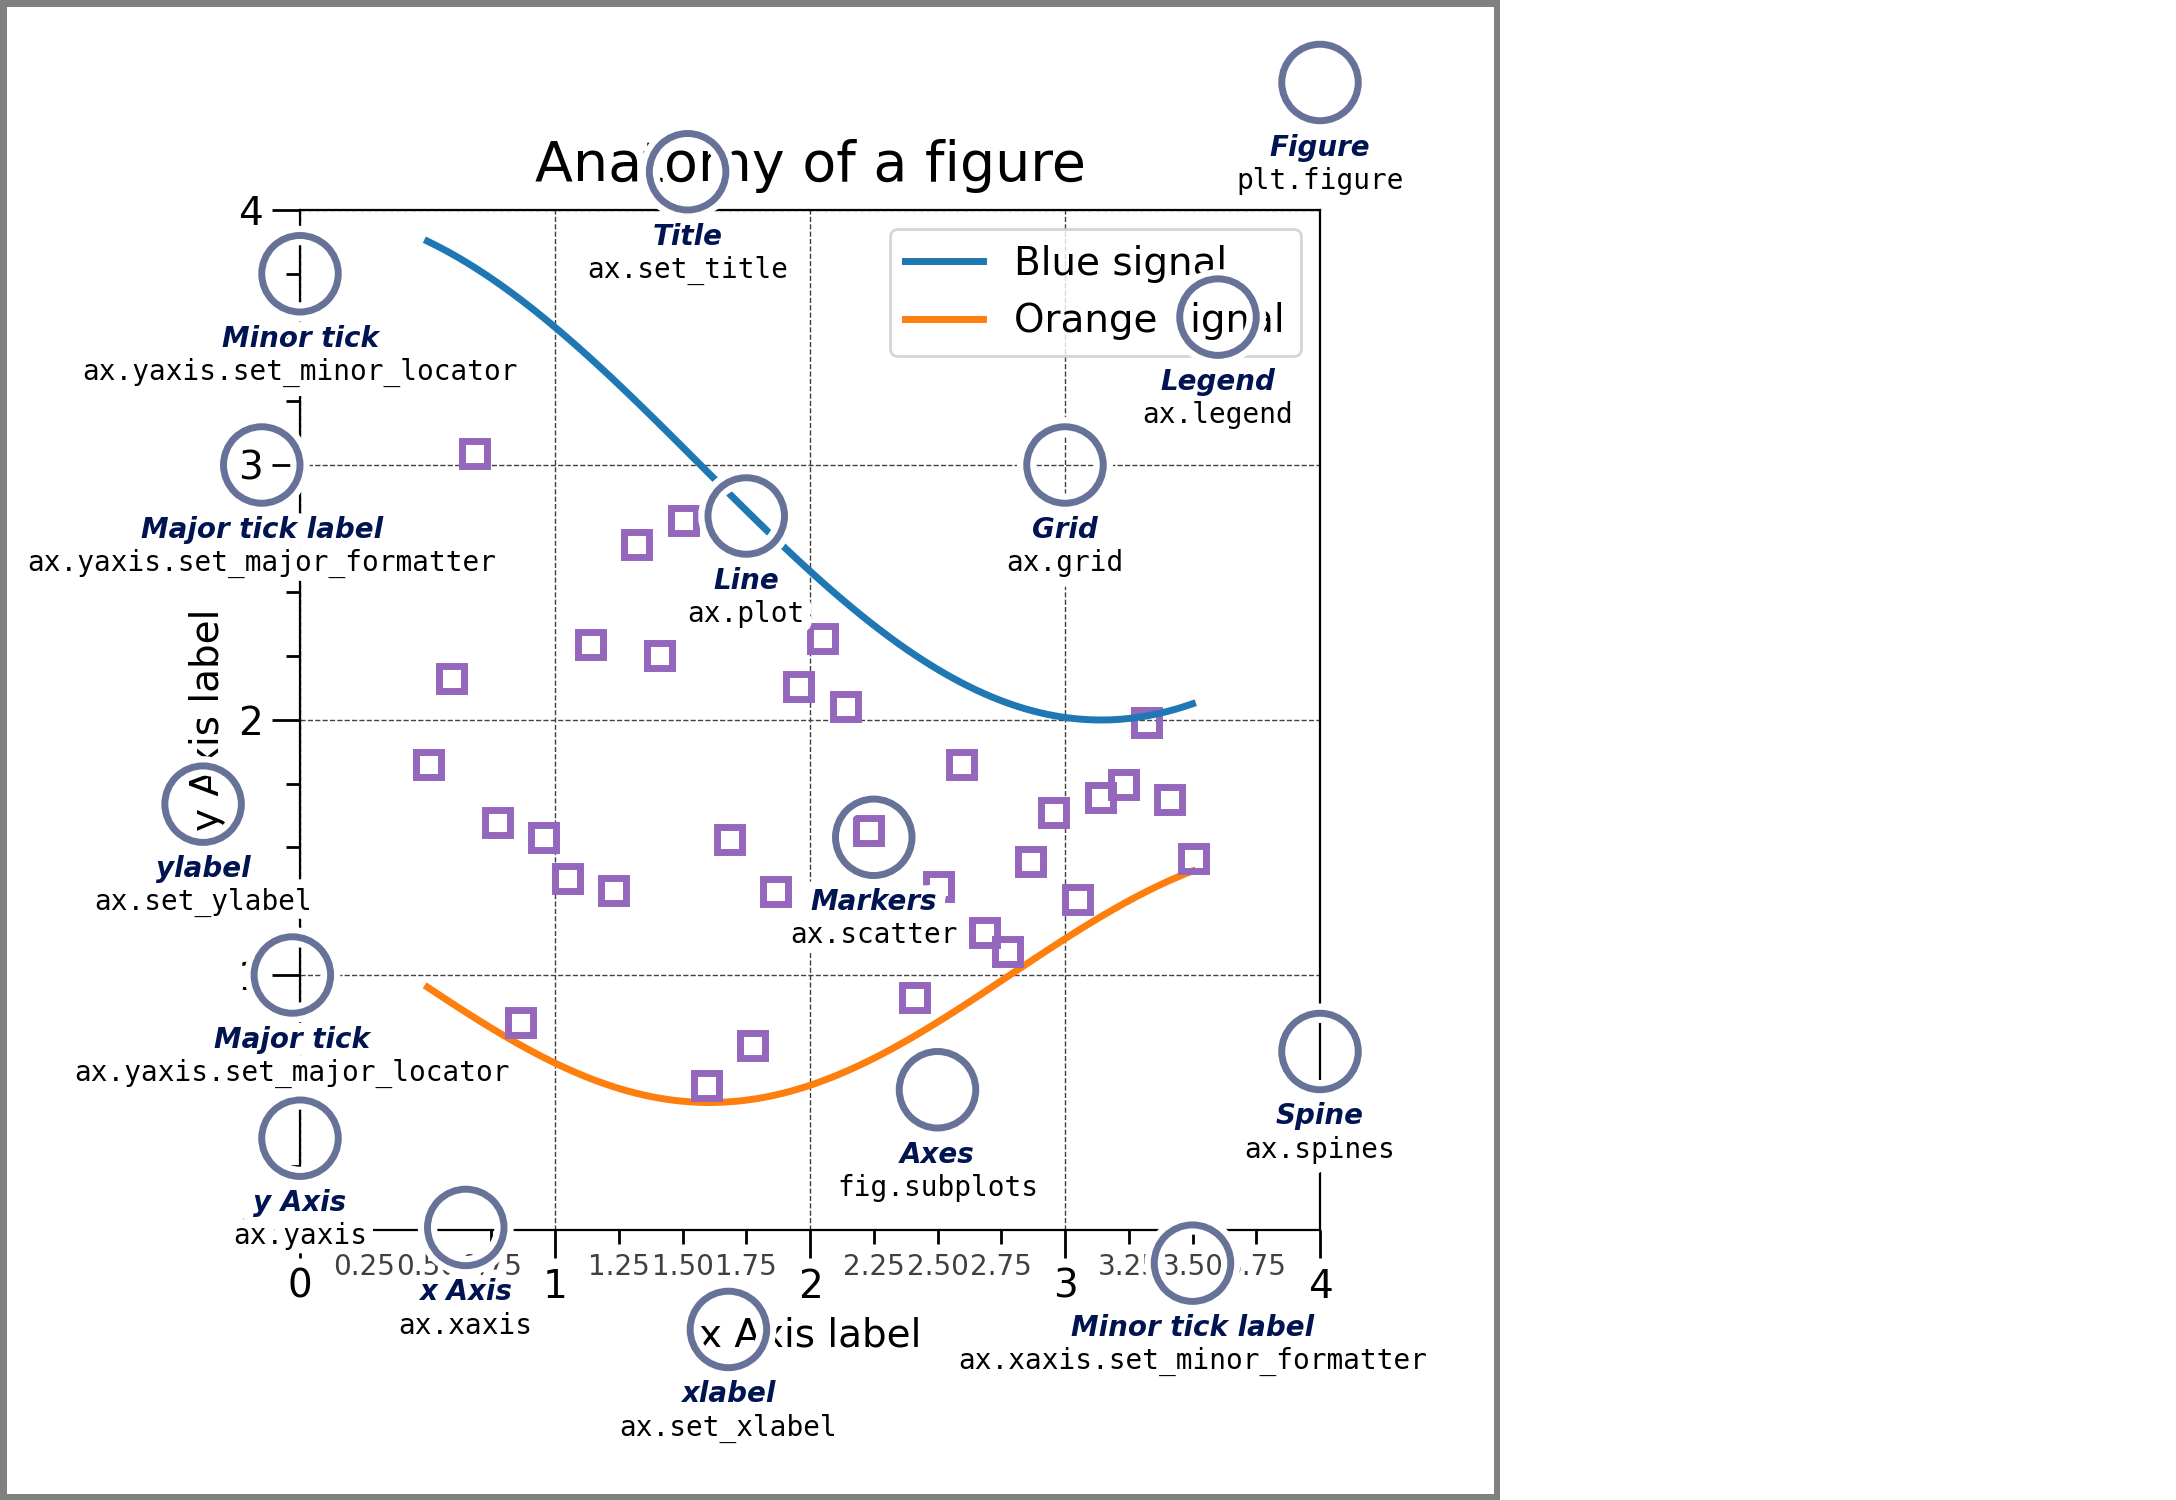
\includegraphics[scale=0.2]{matplotlib1}
\caption{Cấu trúc của đồ thị trong matplotlib}
\label{fig:matplotlib1}
\end{figure}

\begin{itemize}
\item \textbf{Khai báo thư viện}: 
\begin{lstlisting}[language=Python] 
import numpy as np
\end{lstlisting}

\begin{example}
Một số dạng đồ thị: 
\begin{lstlisting}[language=Python]
    # hist(x)
    x = 4 + np.random.normal(0, 2, 200)
    fig, ax = plt.subplots()
    ax.hist(x, bins=8, linewidth=0.5, edgecolor='white')

    plt.show()
\end{lstlisting}
\begin{figure}[ht!]
\centering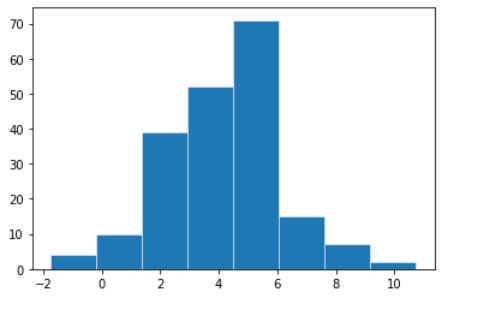
\includegraphics[scale=1]{hist}
\caption{Đồ thị hist}
\label{fig:hist}
\end{figure}
\end{example}

\begin{example}
Một số dạng đồ thị:
\begin{lstlisting}[language=Python]
    # scatter(x, y)
    x = np.random.normal(0, 2, 30)
    y = 4 + np.random.normal(0, 2, 30)
    # Chỉ định kích thước và màu sắc cho đồ thị được vẽ.
    sizes = np.random.uniform(15, 80, 30)
    colors =  np.random.uniform(15, 80, 30)
    fig, ax = plt.subplots()
    ax.scatter(x, y, s=sizes, c=colors, vmin=0, vmax=100)
    plt.show()
\end{lstlisting}
\begin{figure}[ht!]
\centering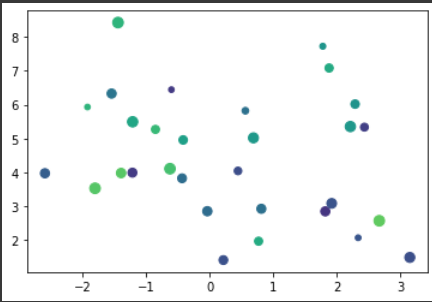
\includegraphics[scale=0.8]{scatter}
\caption{Đồ thị scatter}
\label{fig:scatter}
\end{figure}
\end{example}

\end{itemize}
\subsection{Seaborn}
Seaborn cũng là một thư viện của Python giúp vẽ các đồ thị với sự trợ giúp của Matplotlib, Numpy và Pandas. Nó có thể
được coi là một phần mở rộng của một thư viện Matplotlib vì nó được xây dựng dựa trên đó. Seaborn giúp quan sát các biến dữ liệu dạng đơn trị và đa trị.
Nó còn có các đồ thị rất trực quan và đẹp mắt.

Cài đặt và khai báo seaborn:
\begin{itemize}
    \item Sử dụng Command Prompt: 
    \begin{lstlisting}[language=Python]
        pip install seaborn
    \end{lstlisting}
    \item Hoặc sử dụng Anaconda Prompt:
    \begin{lstlisting}[language=Python]
        conda install seaborn
    \end{lstlisting}
    \item Khai báo thư viện:
    \begin{lstlisting}[language=Python]
        import seaborn as sns
    \end{lstlisting}
\end{itemize}

\begin{example}
Ví dụ đồ thị:
\begin{lstlisting}[language=Python]
penguins = sns.load_dataset('penguins')
sns.histplot(data=penguins, x='flipper_length_mm', hue='species', multiple='stack')
\end{lstlisting}
\begin{figure}[ht!]
\centering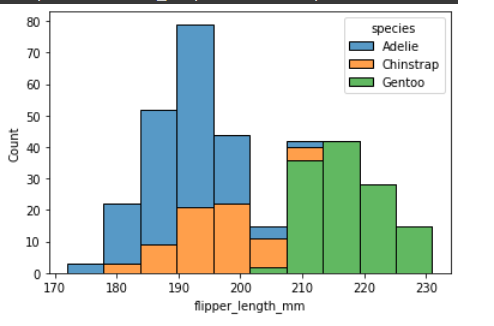
\includegraphics[scale=0.6]{seaborn}
\caption{Đồ thị trong seaborn}
\label{fig:seaborn}
\end{figure}
\end{example}
\end{document}